\documentclass[12pt,letterpaper]{article}
\usepackage{graphicx,textcomp}
\usepackage{natbib}
\usepackage{setspace}
\usepackage{fullpage}
\usepackage{color}
\usepackage[reqno]{amsmath}
\usepackage{amsthm}
\usepackage{fancyvrb}
\usepackage{amssymb,enumerate}
\usepackage[all]{xy}
\usepackage{endnotes}
\usepackage{lscape}
\newtheorem{com}{Comment}
\usepackage{float}
\usepackage{hyperref}
\newtheorem{lem} {Lemma}
\newtheorem{prop}{Proposition}
\newtheorem{thm}{Theorem}
\newtheorem{defn}{Definition}
\newtheorem{cor}{Corollary}
\newtheorem{obs}{Observation}
\usepackage[compact]{titlesec}
\usepackage{dcolumn}
\usepackage{tikz}
\usetikzlibrary{arrows}
\usepackage{multirow}
\usepackage{xcolor}
\newcolumntype{.}{D{.}{.}{-1}}
\newcolumntype{d}[1]{D{.}{.}{#1}}
\definecolor{light-gray}{gray}{0.65}
\usepackage{url}
\usepackage{listings}
\usepackage{color}

\definecolor{codegreen}{rgb}{0,0.6,0}
\definecolor{codegray}{rgb}{0.5,0.5,0.5}
\definecolor{codepurple}{rgb}{0.58,0,0.82}
\definecolor{backcolour}{rgb}{0.95,0.95,0.92}

\lstdefinestyle{mystyle}{
	backgroundcolor=\color{backcolour},   
	commentstyle=\color{codegreen},
	keywordstyle=\color{magenta},
	numberstyle=\tiny\color{codegray},
	stringstyle=\color{codepurple},
	basicstyle=\footnotesize,
	breakatwhitespace=false,         
	breaklines=true,                 
	captionpos=b,                    
	keepspaces=true,                 
	numbers=left,                    
	numbersep=5pt,                  
	showspaces=false,                
	showstringspaces=false,
	showtabs=false,                  
	tabsize=2
}
\lstset{style=mystyle}
\newcommand{\Sref}[1]{Section~\ref{#1}}
\newtheorem{hyp}{Hypothesis}

\title{Problem Set 1}
\date{Due: October 8, 2026}
\author{Applied Stats/Quant Methods 1}

\begin{document}
	\maketitle
	
	\section*{Instructions}
	\begin{itemize}
	\item Please show your work! You may lose points by simply writing in the answer. If the problem requires you to execute commands in \texttt{R}, please include the code you used to get your answers. Please also include the \texttt{.R} file that contains your code. If you are not sure if work needs to be shown for a particular problem, please ask.
\item Your homework should be submitted electronically on GitHub.
\item This problem set is due before 23:59 on Thursday October 8, 2026. No late assignments will be accepted.
	\end{itemize}
	
	\vspace{1cm}
	\section*{Question 1: Education}

A school counselor was curious about the average of IQ of the students in her school and took a random sample of 25 students' IQ scores. The following is the data set:\\
\vspace{.5cm}

\lstinputlisting[language=R, firstline=36, lastline=36]{PS01_answers_JX.R}  


\vspace{1cm}

\begin{enumerate}
	\item Find a 90\% confidence interval for the average student IQ in the school (As a hint, you first need the mean and SD to create a CI):\\
	
	
	\begin{doublespace}
	\textbf{Answer:}\\
	Find mean, standard deviation and standard error in R.
	\lstinputlisting[language=R, firstline=39, lastline=44]{PS01_answers_JX.R}
	
	Sample size is less than 30, use t-distribution.
	\lstinputlisting[language=R, firstline=46, lastline=47]{PS01_answers_JX.R}
	In above function $qt()$, the argument $p$ = 1 - 0.1/2 = 0.95
	
	\lstinputlisting[language=R, firstline=48, lastline=51]{PS01_answers_JX.R}
	\end{doublespace}

	\item Next, the school counselor was curious  whether  the average student IQ in her school is higher than the average IQ score (100) among all the schools in the country.\\ 
	
	\noindent Using the same sample, conduct the appropriate hypothesis test with $\alpha=0.05$.
	
	\begin{doublespace}
		\textbf{Answer:}\\
		\textbf{Assumption}: data is randomly selected and the population is normally distributed.
		\textbf{Hypothesis}:\\
		$H_0: \mu \leq 100$\\
		$H_A: \mu > 100$\\
		
		\textbf{Calculate test statistics:} \\
		Since the sample size is small we use t-score to calculate test statistic:
		$$t = \frac{\bar{y} - \mu_0}{\sigma_{\bar{y}}}$$
		We can find $t$ in R.
		\lstinputlisting[language=R, firstline=59, lastline=60]{PS01_answers_JX.R}
		
		\textbf{Calculate P-value in R:}
		\lstinputlisting[language=R, firstline=63, lastline=64]{PS01_answers_JX.R}
		
		\textbf{Conclusion}:\\
		Since P-value $>\alpha(0.05)$, we fail to reject the null hypothesis. There is insufficient evidence to conclude that the average student IQ in this school is greater than the average IQ score of 100 among all schools in the country.
	\end{doublespace}
\end{enumerate}

\newpage

	\section*{Question 2: Political Economy}

\noindent Researchers are curious about what affects the amount of money communities spend on addressing homelessness. The following variables constitute our data set about social welfare expenditures in the USA. \\
\vspace{.5cm}


\begin{tabular}{r|l}
	\texttt{State} &\emph{50 states in US} \\
	\texttt{Y} & \emph{per capita expenditure on shelters/housing assistance in state}\\
	\texttt{X1} &\emph{per capita personal income in state} \\
	\texttt{X2} &  \emph{Number of residents per 100,000 that are "financially insecure" in state}\\
	\texttt{X3} &  \emph{Number of people per thousand residing in urban areas in state} \\
	\texttt{Region} &  \emph{1=Northeast, 2= North Central, 3= South, 4=West} \\
\end{tabular}

\vspace{.5cm}
\noindent Explore the \texttt{expenditure} data set and import data into \texttt{R}.
\vspace{.5cm}
\lstinputlisting[language=R, firstline=72, lastline=72]{PS01_answers_JX.R}  
\vspace{.5cm}
\begin{itemize}

\item
Please plot the relationships among \emph{Y}, \emph{X1}, \emph{X2}, and \emph{X3}? What are the correlations among them (you just need to describe the graph and the relationships among them)?
\vspace{.5cm}
\begin{doublespace}
	\textbf{Answer:}\\
	First, plot scatter plot to show the relationship between \emph{Y}(per capita expenditure on shelters/housing assistance in state) and \emph{X1}(per capita personal income in state).
\end{doublespace}

\item
Please plot the relationship between \emph{Y} and \emph{Region}? On average, which region has the highest per capita expenditure on housing assistance?\\
\begin{doublespace}
	\textbf{Answer:}\\
	To make the number from Region easier to be understood. I can change Region to factor with label names of Northeast, North Central, South and West.
	\lstinputlisting[language=R, firstline=135, lastline=137 ]{PS01_answers_JX.R}
	
	Then create scatter plot.
	\lstinputlisting[language=R, firstline=139, lastline=146 ]{PS01_answers_JX.R}
	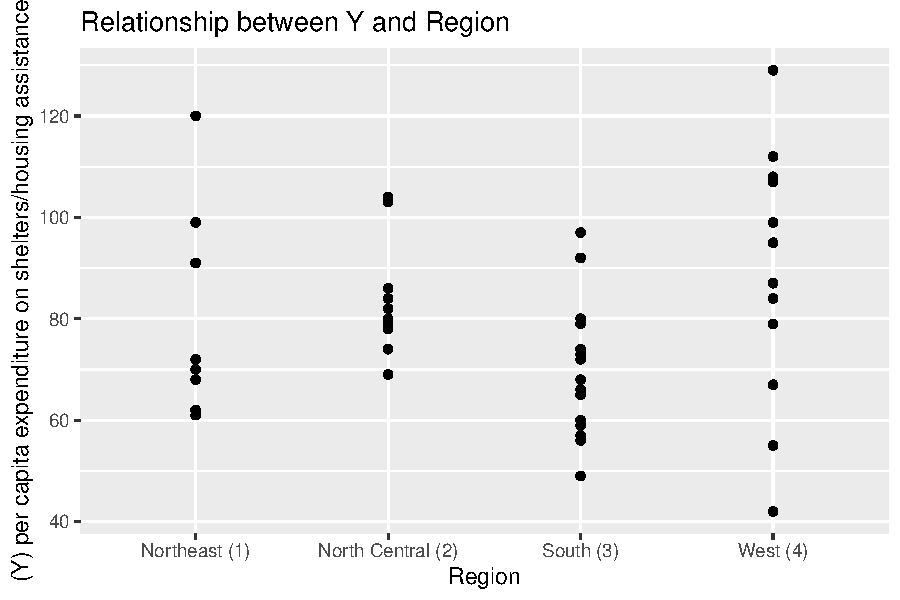
\includegraphics[width=0.6\textwidth]{y_region_scatter.pdf}\\
	
	To find the average, I can use box plot to compare the mean per capita expenditure among different region.
	\lstinputlisting[language=R, firstline=153, lastline=164 ]{PS01_answers_JX.R}
	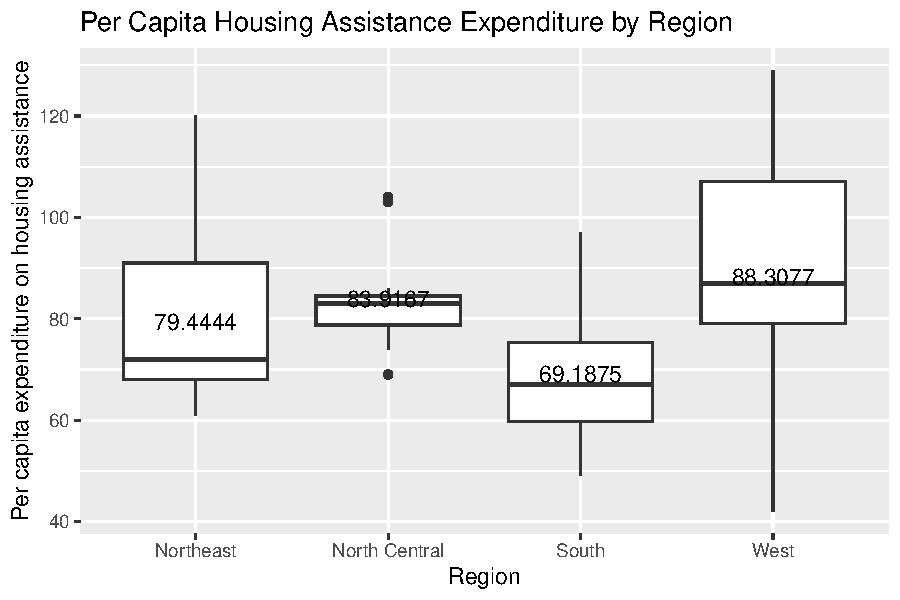
\includegraphics[width=0.6\textwidth]{y_region_box.pdf}\\
	
	On average, US states that are categorized as "West" has the highest per capita expenditure on housing assistance. With 88.3077.
	
\end{doublespace}
\vspace{.5cm}
\item
Please plot the relationship between \emph{Y} and \emph{X1}? Describe this graph and the relationship. Reproduce the above graph including one more variable \emph{Region} and display different regions with different types of symbols and colors. \\
\begin{doublespace}
	\textbf{Answer:}\\
	\lstinputlisting[language=R, firstline=81, lastline=88 ]{PS01_answers_JX.R}
	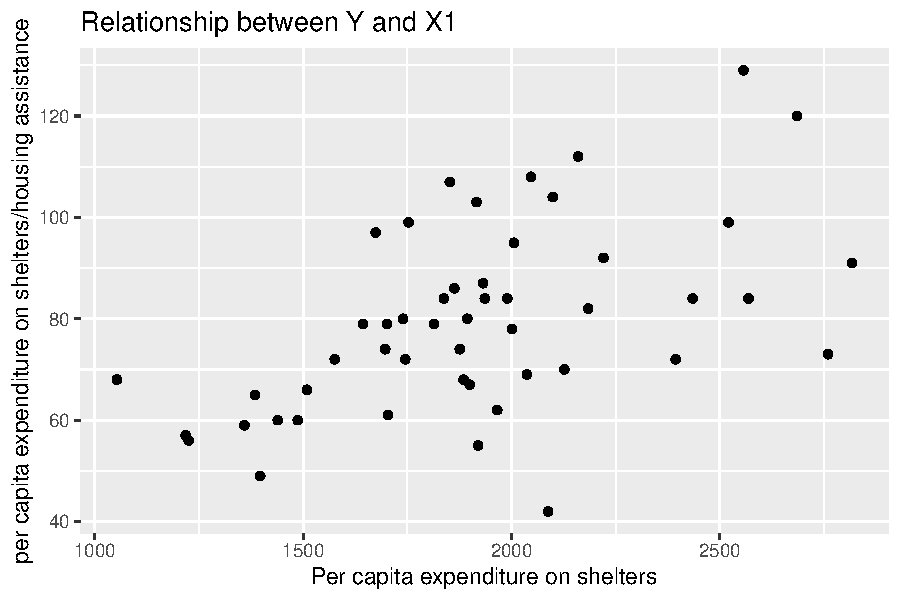
\includegraphics[width=0.8\textwidth]{Y_X1.pdf}
	In the above graph, Y and X1 have a positive, weak, and linear association.
	
\end{doublespace}
\end{itemize}


\end{document}
